% Subsections 1--2 of the distributed section (input from distributed.tex).

\subsection{Distributed histories}
\label{sec:histories}

Until now, runs have been independent: each state changes only through that
run's input and output events.  We now place one such run at each participant in
a finite set $\mathcal N$ of any size.  Participant $p$ starts in the canonical state
$\sigma_P(i_p)$ and still changes its state only through its own specification
events.  The new ingredient is communication.  Besides learning input directly
from the environment, a participant can learn cumulative input from another
participant.

Participants exchange messages by $\mathsf{send}(m)$ and
$\mathsf{receive}(m)$.  A \emph{message} $m=(j,d)$ carries a cumulative input $j$, or $\varnothing$ if it
carries none, and application-specific data $d$, such as timestamps, version
vectors, or state identifiers (described below).  Receiving a message does not
change the specification state.  A participant at $(i,R)$ that receives $(j,d)$ with
$j\neq\varnothing$ may incorporate $j$ by its own $\mathsf{input}(k)$ for a
legal common \indesc $k$ of $i$ and $j$, when one exists.  The system chooses $k$; the data $d$ can influence that choice but never
changes the state directly.

Send and receive events connect the participants' locally ordered runs.  Adding
an edge from each send to its matching receive gives the standard model of a
distributed history; the transitive closure of these edges and the local orders
is happens-before.

\begin{definition}[Distributed history, history event]
\label{def:distributed-history}
Fix an \spectype, participants $\mathcal N$, and an initial input $i_p$
for each.  A \emph{distributed history} $H$ is a finite set of
\emph{history events}, each an occurrence at one participant of a
specification event (Definition~\ref{def:run}), $\mathsf{send}(m)$, or
$\mathsf{receive}(m)$, with:
\begin{enumerate}
  \item a total local order on each participant's history events;
  \item for each receive, a matching send of the same message at another
        participant, each send matching at most one receive;
  \item for each participant $p$, its specification events, in local order,
        form a defined transition sequence from $\sigma_P(i_p)$: each
        is legal at the state where it occurs; and
    \item no history event happens before itself.
\end{enumerate}
\end{definition}

\begin{definition}[Happens-before]
\label{def:happens-before}
\emph{Happens-before} is the transitive closure of the local orders of a
distributed history and of each send preceding its matching receive.
\end{definition}

\begin{definition}[Consistent cut]
\label{def:consistent-cut}
A \emph{consistent cut} $C$ is a subset of history events closed under happens-before~\cite{lamport1978time,chandy1985distributed}.  The term is standard and unrelated to our notion of consistency.
\end{definition}

A consistent cut contains a prefix of each participant's history events, so by
item~3
it determines one run per participant.

\begin{definition}[Participant run]
\label{def:participant-run}
At a consistent cut $C$, the specification events of $C$ at participant $p$,
in local order, form its \emph{participant run}, a run
(Definition~\ref{def:run}) whose final state we write $\sigma_p(C)$.
\end{definition}

\begin{definition}[Endpoint]
\label{def:endpoint}
The \emph{endpoint} of a consistent cut $C$ is
$\operatorname{end}(H,C)=(\sigma_p(C))_{p\in\mathcal N}$.
\end{definition}

\begin{figure}[t]
  \centering
  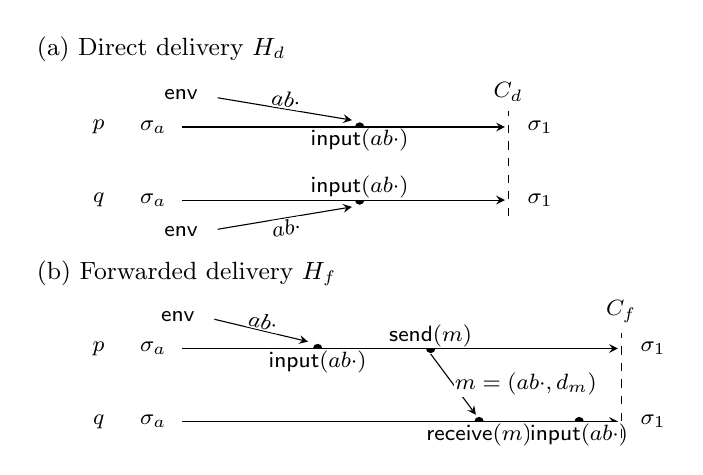
\begin{tikzpicture}[x=.82cm,y=.58cm,>=stealth,
                      every node/.style={font=\footnotesize}]
    % Direct delivery.
    \node[anchor=west,font=\small] at (-1,7.2) {(a) Direct delivery $H_d$};
    \node[anchor=east] at (.35,5.5) {$p$};
    \node[anchor=east] at (.35,3.9) {$q$};
    \node[anchor=west] at (.6,5.5) {$\sigma_a$};
    \node[anchor=west] at (.6,3.9) {$\sigma_a$};
    \draw[->] (1.4,5.5) -- (6.4,5.5);
    \draw[->] (1.4,3.9) -- (6.4,3.9);
    \fill (4.15,5.5) circle (1.7pt);
    \fill (4.15,3.9) circle (1.7pt);
    \node[below,fill=white,inner sep=.5pt] at (4.15,5.5)
      {$\mathsf{input}(ab\cdot)$};
    \node[above,fill=white,inner sep=.5pt] at (4.15,3.9)
      {$\mathsf{input}(ab\cdot)$};
    \node[anchor=east] at (1.8,6.2) {$\mathsf{env}$};
    \node[anchor=east] at (1.8,3.2) {$\mathsf{env}$};
      \draw[->] (1.95,6.14) -- node[midway,above,sloped,fill=white,inner sep=.5pt]
        {$ab\cdot$} (4.03,5.65);
      \draw[->] (1.95,3.26) -- node[midway,below,sloped,fill=white,inner sep=.5pt]
        {$ab\cdot$} (4.03,3.75);
    \draw[dashed] (6.45,3.55) -- (6.45,5.85);
    \node[above] at (6.45,5.85) {$C_d$};
    \node[anchor=west] at (6.6,5.5) {$\sigma_1$};
    \node[anchor=west] at (6.6,3.9) {$\sigma_1$};

    % Forwarded delivery.
    \node[anchor=west,font=\small] at (-1,2.3) {(b) Forwarded delivery $H_f$};
    \node[anchor=east] at (.35,.65) {$p$};
    \node[anchor=east] at (.35,-.95) {$q$};
    \node[anchor=west] at (.6,.65) {$\sigma_a$};
    \node[anchor=west] at (.6,-.95) {$\sigma_a$};
    \draw[->] (1.4,.65) -- (8.15,.65);
    \draw[->] (1.4,-.95) -- (8.15,-.95);
    \node[anchor=east] at (1.75,1.35) {$\mathsf{env}$};
      \draw[->] (1.9,1.29) -- node[midway,above,sloped,fill=white,inner sep=.5pt]
        {$ab\cdot$} (3.35,.8);
    \fill (3.5,.65) circle (1.7pt);
    \node[below,fill=white,inner sep=.5pt] at (3.5,.65)
      {$\mathsf{input}(ab\cdot)$};
    \fill (5.25,.65) circle (1.7pt);
    \node[above,fill=white,inner sep=.5pt] at (5.25,.65)
      {$\mathsf{send}(m)$};
    \fill (6.0,-.95) circle (1.7pt);
    \node[below,fill=white,inner sep=.5pt] at (6.0,-.95)
      {$\mathsf{receive}(m)$};
    \draw[->] (5.25,.53) -- node[midway,right,fill=white,inner sep=.5pt]
      {$m=(ab\cdot,d_m)$} (5.95,-.8);
    \fill (7.55,-.95) circle (1.7pt);
    \node[below,fill=white,inner sep=.5pt] at (7.55,-.95)
      {$\mathsf{input}(ab\cdot)$};
    \draw[dashed] (8.2,-1.3) -- (8.2,1.0);
    \node[above] at (8.2,1.0) {$C_f$};
    \node[anchor=west] at (8.35,.65) {$\sigma_1$};
    \node[anchor=west] at (8.35,-.95) {$\sigma_1$};
  \end{tikzpicture}
  \caption{Two histories from $\sigma_a=\sigma_P(a\cdot\cdot)=(a\cdot\cdot,R_0)$ to
  $\sigma_1=(ab\cdot,R_1)$, with $R_0$ and $R_1$ the tables of
  Figure~\ref{fig:election-frames}(a) and~(b).  In (a) each participant records
  $\mathsf{input}(ab\cdot)$ directly; in (b) $q$ records it after receiving $m$.  Dashed lines are consistent cuts.}
  \label{fig:participant-runs}
\end{figure}

In Figure~\ref{fig:participant-runs}, the input $ab\cdot$ reaches $q$
directly or through a message from $p$.  The histories differ, but at either
cut each participant run is $\mathsf{input}(ab\cdot)$, so both endpoints are
$(\sigma_1,\sigma_1)$.

\subsection{Distributed consistency}
\label{sec:distributed-consistency}

A \emph{continuation} of a history at a consistent cut $C$ is a history $H'$
that extends the history events of $C$ with further history events after
them.  All of $H'$ is a consistent cut of $H'$, its \emph{final cut}.  Let $j$ be a common \indesc of the participants' current inputs at a consistent cut $C$.  The cut $C$ is \emph{confluent at} $j$ when some continuation at $C$ has a final cut with endpoint $\bigl((j,R)\bigr)_{p\in\mathcal N}$ for some $R$, so that every participant ends in the same state $(j,R)$.  History events at different participants are independent, so this holds exactly when the participant runs at $C$ are
confluent at $j$ (Definition~\ref{def:consistency}).

\begin{definition}[Consistency of distributed histories]
\label{def:distributed-consistency}
The distributed histories of an \spectype are \emph{consistent} when, for every
finite participant set, every consistent cut of every history is confluent
at every common \indesc of the participants' current inputs.
\end{definition}

\begin{proposition}[Distributed consistency]
\label{prop:distributed-consistency}
The runs of an \spectype are consistent if and only if its distributed
histories are consistent.
\end{proposition}

\begin{proof}[Proof sketch]
First assume the runs are consistent.  The participant runs at a cut are a
finite family of runs, so every cut is confluent at every common \indesc, and the histories are
consistent.  Now assume the histories are consistent.  Any finite family of
runs is the set of participant runs at the final cut of a history whose
participants exchange no messages, so the runs are consistent.  Full proof in
Appendix~\ref{app:proofs-sec4}.
\end{proof}

By Complete CALM, which reduces to Functional CALM with one output per input,
the distributed histories of a spec are consistent exactly when the spec
satisfies Lifted Monotonicity.  For specs with Lifted Monotonicity, the Survivor test
(Proposition~\ref{prop:confluence}) gives a row $(j,u)$ that every participant's
state still contains, where $j$ is a common \indesc of all participants' current
inputs; by Lemma~\ref{lem:run-residual}, $u$ \outrel everything they have
emitted.  Each participant can then perform $\mathsf{input}(j)$ and
$\mathsf{output}(u)$ and reach the same state without \commitment
(Proposition~\ref{prop:exposure-boundary}).  The spec guarantees only that such
a $u$ exists; choosing it, communicating it, and scheduling the events are left
to the system.

For functional specs,
Corollary~\ref{cor:state-by-input} also gives convergence:

\begin{corollary}[Convergence]
\label{cor:convergence}
In any history of a monotone functional specification, every
participant whose current input at a consistent cut is $j$ is in state
$\sigma_P(j)$.  Participants with the same current input therefore agree,
regardless of message paths, arrival order, or the outputs they emitted.
\end{corollary}

\begin{proof}
Each participant run is a run, so Corollary~\ref{cor:state-by-input} applies.
\end{proof}

With several outputs per input, convergence can fail even when the spec
satisfies Lifted Monotonicity.  In Figure~\ref{fig:ambiguity-frames}(g), a run at input $\{\texttt{s}\}$ that emitted
$\{\texttt{s}{\to}\texttt{s1}\}$ has subsumed the route sets that leave it out, while a run at the same input that
emitted nothing keeps them.  Consistency then guarantees only that such participants can be reconciled, not
that they agree.

\paragraph{Message data.}
The data $d$ of a message is any application state other than input that a
participant chooses to send, such as timestamps, version vectors, gossip, or votes.  Data
can influence which history events occur next at the receiver, but can
never directly change the receiver's specification state, and nothing in the
definitions above depends on it.
Participants may also share emitted outputs in $d$; this does not change
at which inputs a cut is confluent (Appendix~\ref{app:exchanging-outputs}).
